\chapter{Background Literature}\label{chap:lit}
\begin{overview}
  A literature overview on model predictive control and controller constraints
  is presented in this chapter. Process operability is reviewed and the
  operability index -- used as the basis for constraint interaction -- is 
  defined. Finally, a summary of the mathematical techniques used is given.
\end{overview}

\section{Model Predictive Control}
Since its successful implementation in the petrochemical industry, model
predictive control (MPC) has gained widespread acceptance in the processing 
sector \citep[1]{maciejowskimpc}. This has led to the development of many 
commercial MPC packages such as DMCplus (Aspentech), RMPCT (Honeywell),
Connoisseur (Invensys) and SMOC (Shell Global Solutions) \citep{qinbadgwell}.
\subsection{Control theory}
Model predictive control differs from other model based control techniques (such
 as Inverse Nyquist Array- and Internal Model Control) in its active use of 
predictions for future process outcomes \citep[137]{maciejowskifb}. In this 
context, MPC further distinguishes itself from other predictive control
techniques in its ability to accommodate constraints on inputs and outputs.

\citet[8]{maciejowskimpc} summarises the control methodology of MPC in four 
steps; Measure, Predict, Optimize/Calculate and Apply. Along with 
figure~\ref{fig:mpc:general} these steps are summarized below;
%TODO - add symbols to list
\begin{enumerate}
  \item Measure; the current outputs are measured and the error (deviation from
    the set-point trajectory) is calculated.
  \item Predict; using the model, future outputs are calculated (over the 
    prediction horizon).
  \item Optimize/Calculate; control moves (over the control horizon) are now
    calculated to minimize the predicted deviation from the set-point trajectory.
  \item Apply; only the first control move is implemented, where-after this 
    procedure is restarted.
\end{enumerate}
\begin{figure}[htbp]
  \centering
  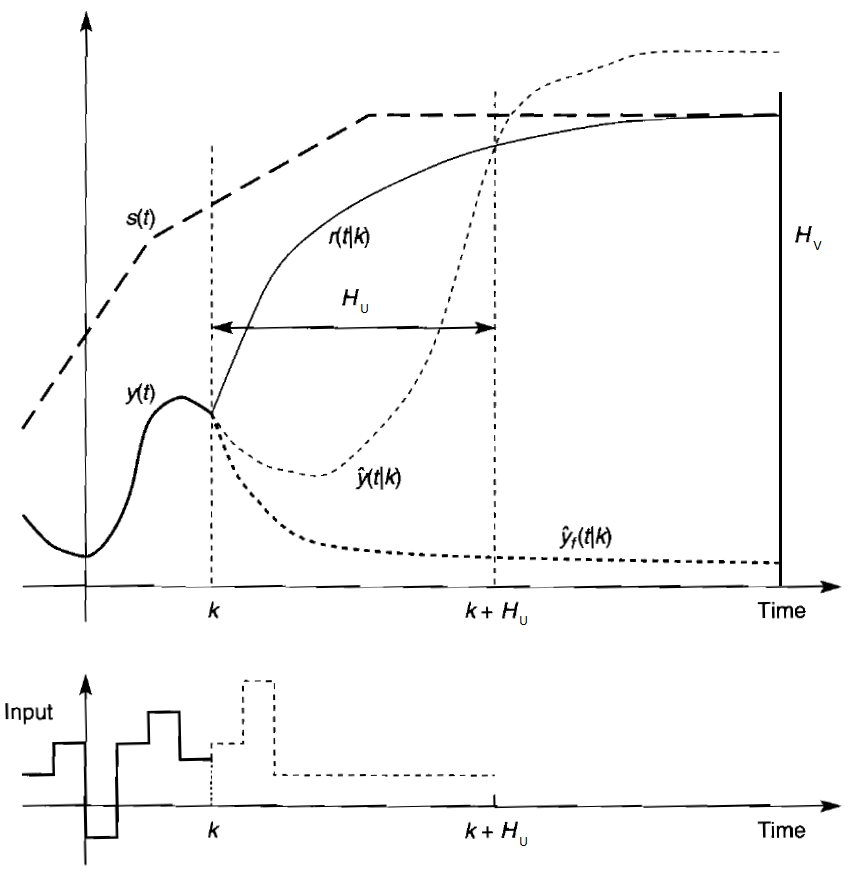
\includegraphics[width=8cm]{graph/mpc_general}
  \caption[General MPC working]{General MPC working, showing predictions on both outputs and inputs}
  \label{fig:mpc:general}
%TODO - fix figure to use coherent nomenclature
\end{figure}

\subsection{Objective functions}
Optimal control moves are determined by means of objective functions. These 
functions are often referred to as cost functions \citep[41]{maciejowskimpc} as
they can incorporate input/output weighting based on economic factors.

The general formulation of the unconstrained objective function is presented in
equation~\ref{eq:genobjfn}. Modifications to this function (due to constraints)
is discussed in section~\ref{sec:conobjfn}. From \citet[17]{rawlings} and
\citet[41]{maciejowskimpc}, the objective function which penalizes deviations
from the set-point trajectory as well as moves in the inputs is shown below;
% TODO - eqn in terms of zero setpoint, generalize to non-zero sp
\begin{equation}
  \label{eq:genobjfn}
  V(x(0),{\bf u})=\frac{1}{2}\sum^{N-1}_{k=0}[x(k)'Qx(k)+u(k)'Ru(k)]
  + \frac{1}{2}x(N)'P_fx(N)
\end{equation}
It is clear that the objective function depends on both the state sequence and
the input sequence. The current state, $x(0)$ is known (measured) and the 
subsequent states are determined by the model and the input sequence. The
optimal MPC control problem therefore becomes;
\begin{equation}
  \label{eq:opctrlprob}
  \min_{\bf u} V(x(0),{\bf u})
\end{equation}
\subsection{Models}
\subsubsection{Impulse response models}
\subsubsection{Pulse response models}
\subsubsection{Other model types}
\subsection{Tuning}
As far as the objective function (equation~\ref{eq:genobjfn}) is concerned, the
most prominent tuning parameters for MPC is the weighting matrices $Q$, $R$ and
$P_f$. These are used to enforce the relative importance of deviations in both
the inputs and outputs.

The weighting matrices are by no means the only tuning parameters for MPCs;
additional parameters include the horizons used for predictions, the reference
trajectory and the auxiliary models used (e.g. disturbance models). Chapter 7
of \citet{maciejowskimpc} covers the tuning of MPCs in some detail.

\section{Constraints in MPC}
When used in conjunction with a steady-state optimizer, MPCs are able to operate
with more CVs than MVs \citet{vinsonphd}. Control of the CVs are now within
ranges rather than on set-points.
\subsection{Constrained objective functions}\label{sec:conobjfn}
\subsection{Control constraints}
\subsection{Optimization constraints}

\subsection{Effect on models}
\subsection{Effect on solutions}

\section{Process Operability}
The method of constraint handling, as presented in this document, stems largely
from work done by Georgakis and colleagues, in particular \citet{vinsonphd},
\citet{vinsonartoi}, \citet{limaphd}, \citet{opconproc} and \citet{opidealrx}.
The following sections give an overview of process operability techniques
and proceeds to clearly define operability index of \citet{vinsonphd}.
\subsection{Overview}
\subsection{Operability Index}
The operability index was defined by \citet{vinsonphd} as a measure of steady-
state process operability. Constraint interdependence is used as the basis of
this index. Further work by \citet{limaphd} expanded this index to dynamic
systems. This expansion, however, only focuses on a specific class of dynamic
behavior and cannot be considered optimal.
%% EXPAND
\subsubsection{Definitions}
The operability index focuses on input-output relationships rather the system's
dynamic states \citep{vinsonphd}. Input and output values are defined by
'spaces' (in $R^n$). These spaces are the 'feasible regions' which are 
bounded by the inequalities describing the ranges of the inputs or outputs. The
following spaces are of interest;
\begin{itemize}
  \item Available Input Space (AIS); the set of values that process inputs can
    take. The limits on these values are based on both physical limits (e.g.
    valve openings) or process design values (e.g. flow-rates or temperatures).
    Figure \ref{fig:sampleais} illustrates an AIS for two variables ($u_1, u_2$)
    bounded by simple high/low limits.
  \item Achievable Output Space (AOS); this is the set of values which the 
    process outputs can obtain, given the AIS. The AIS maps to the AOS by means
    of a process model, $G$. Therefore, a point $u$ in the AIS corresponds to
    a point $y$ in the AOS via $y=G(u)$. Examples of AOSs for linear and
    non-linear models are shown in figure \ref{fig:sampleaos}.
  \item Desired Output Space (DOS); this represents the desired output values of
    the process. These values are typically based on operational and financial
    parameters. Figure \ref{fig:sampledos} shows a sample DOS for a two output
    system.
  \item Expected Disturbance Space (EDS); all the values of the expected 
    disturbances to the system. In the case of linear models, these values are 
    translated back to the input space by means of a disturbance model, $G_d$.
  \item Desired Input Space (DIS); in the same manner that the AIS maps to the
    AOS, the DIS represents combined reverse mappings of the DOS and EDS. The
    DIS is calculated as the inputs, $u$, that satisfy the model, ie.
    $y=G(u,d)$ (with $y$ and $d$ from the DOS and EDS respectively).Figure 
    \ref{fig:sampledis} shows this combined translation.
\end{itemize}

%% MAYBE USE ONE BIG FIGURE FOR ALL SPACES?
\begin{figure}[htbp]
  \centering
  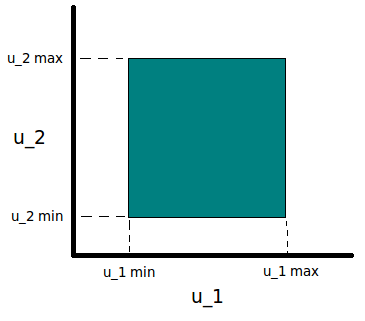
\includegraphics[width=8cm]{graph/sample_ais}
  \caption[Sample Available Input Space]{Sample Available Input Space (AIS) showing high/low limits on both inputs}
  \label{fig:sampleais}
\end{figure}

\begin{figure}[htbp]
  \centering
  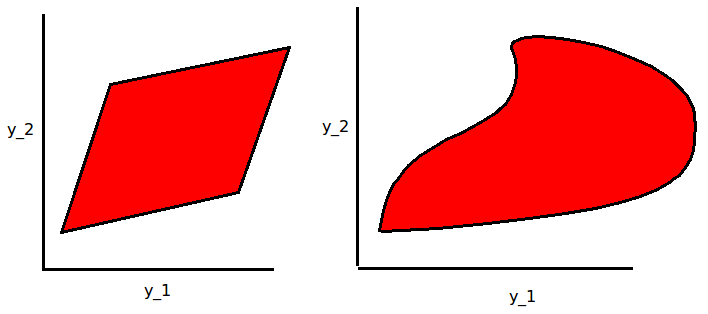
\includegraphics[width=8cm]{graph/sample_aos}
  \caption[Sample Achievable Output Space]{Sample Achievable Output Space (AOS)
    -- Linear model (left) and non-linear model (right)}
  \label{fig:sampleaos}
\end{figure}

\begin{figure}[htbp]
  \centering
  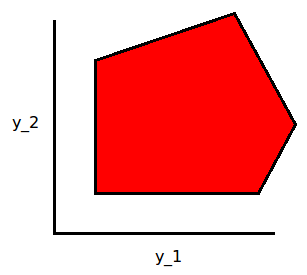
\includegraphics[width=8cm]{graph/sample_dos}
  \caption[Sample Desired Output Space]{Sample Desired Output Space (DOS) with 
    linear constraints on both outputs}
  \label{fig:sampledos}
\end{figure}

\begin{figure}[htbp]
  \centering
  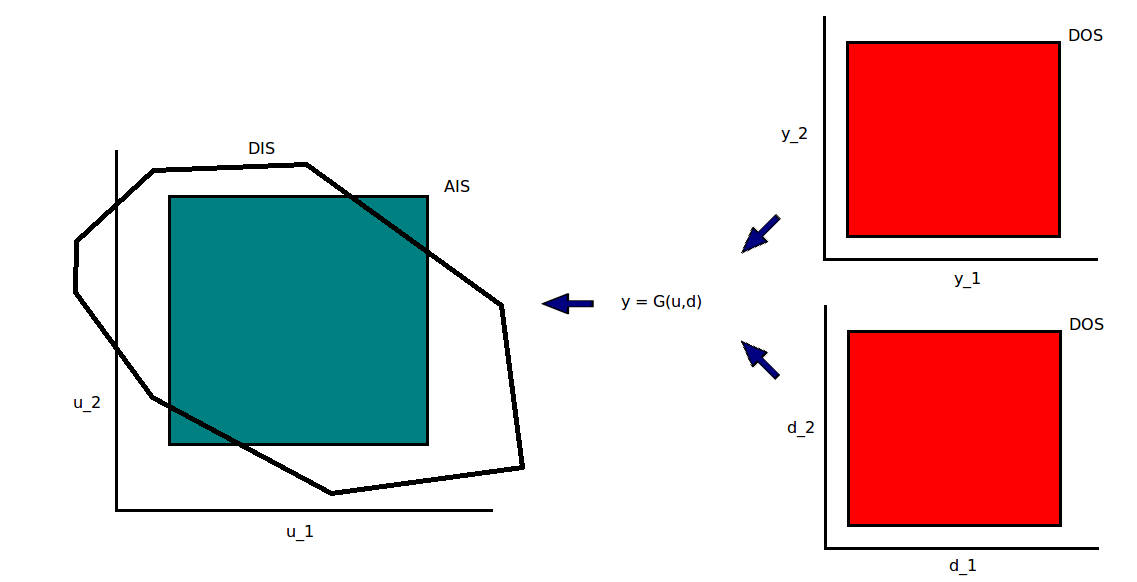
\includegraphics[width=8cm]{graph/sample_dis}
  \caption[Sample Desired Input Space]{Sample Desired Input Space (DIS) for
    a linear model and rectangular DOS and EDS}
  \label{fig:sampledis}
\end{figure}

\citet{vinsonphd} proceeds to define the generalised Output Operability Index
(OOI) as shown in equation \ref{eq:genooi}. Where $\mu$ represents a function
to calculate the volume of a space. From this definition it is clear that the
controlability of a process decreases if the DIS does not cover the whole AIS.
Servo- and regulatory operability indices are also defined in the text, but 
are not shown here.
\begin{equation}
  \label{eq:genooi}
     OOI = \frac{\mu(AIS\cap DIS)}{\mu(DIS)}
\end{equation}

All the concepts above are directly applicable to square systems. For the case
of non-square systems (more outputs than inputs) the operability index
formulation is extended to interval operability. \citet{limaphd} elaborates
on this and defines the following concepts:
[insert Lima]
%% ADD LIMA PHD FORMULATION - CONDENSE!!! %%
% Vinson notes:
% "LP - linear programming"
% "defining the DOS this way will be described as interval/subset operability"
% "As long as DOS intersects AOS, process is operable"
% "Less robust process than when whole AOS lies in DOS."

\subsubsection{Application}
Numerous authors have illustrated the application of the operability index.
%% INSERT OI USE REFS %%

Although the  operability index can be used with square or non-square, linear
or non-linear models, its easiest application is to linear models. This is
advantageous as most of the current MPCs use linear models \citep{vinsonphd}.

\citet{vinsonphd} highlights some properties of MPC (in particular DMCplus)
which lends themselves to the  application of the operability index. 
Table~\ref{tab:mpcoi} summarises these properties and applications.
\begin{table}[htbp]
  \centering
  \caption[Application of the operability index to MPC]{Application of the
    operability index to MPC \citep{vinsonphd}}
  \label{tab:mpcoi}
    \begin{tabular}{p{6cm} p{9cm}}
      \toprule
      MPC property & Operability index property \\
      \midrule
      Linear process models & Calculation of the relevant spaces (AOS and DIS)
                              is usually fast.\\
      Constraints on MVs and 
      CVs                   & In the case of fixed constraints; the input/
                              output constraints result in polytopes in both
                              the input/output spaces. From these descriptions
                              the framework of operability index can be directly
                              applied.\\
      Solution of MV and CV 
      steady state targets  & Where an LP solver is used, the operability index
                              can yield useful information about process
                              characteristics.\\
      \bottomrule
    \end{tabular}
\end{table}

\section{Mathematical Background}
\subsection{Process models}
\subsubsection{Linear}
\subsubsection{Non-linear}
% Polynomial
% (Other)
\subsection{Techniques}
% Topology (etc.)